%%
%% This is file `bjtu-bachelor-thesis.cls'
%%
%% ------------------------------------------------------------------------
%% Copyright (C) 2022 Q.Tang
%% 
%% Licensed under the Apache License, Version 2.0 (the "License");
%% you may not use this file except in compliance with the License.
%% You may obtain a copy of the License at
%% 
%%     http://www.apache.org/licenses/LICENSE-2.0
%% 
%% Unless required by applicable law or agreed to in writing, software
%% distributed under the License is distributed on an "AS IS" BASIS,
%% WITHOUT WARRANTIES OR CONDITIONS OF ANY KIND, either express or implied.
%% See the License for the specific language governing permissions and
%% limitations under the License.
%% ------------------------------------------------------------------------
\documentclass{bjtu-bachelor-thesis}
%========================================================================%
% 自定义内容
%========================================================================%

\author{XX}
\studentNumber{1730xxxx}
\advisor{XXX}
\school{软件学院}
\major{软件工程}
\title{设计(论文)题目}
\englishtitle{The Design and Implementation of \\ Thesis Template Based on \LaTeX}

%========================================================================%
% 前置部分
%========================================================================%

\begin{document}
\pagenumbering{roman}
\makecover % 封面
\makeAuthorization % 版权声明

\setcounter{page}{1}
\pagestyle{bjtufancy}

\begin{chineseabstract}	

\noindent\bjtusongti{\textbf{摘要:}}[鼠标左键单击选择该段落,输入替换之。内容为小四号宋体。] 中文摘要应将论文的内容要点简短明了地表达出来,约400字左右,字体为宋体小四号。内容应包括工作目的、研究方法、成果和结论。要突出本论文的创新点,语言力求精炼。为了便于文献检索,应在本页下方另起一行注明论文的关键词(3-5个),如有可能,尽量采用《汉语主题词表》等词表提供的规范词。图X幅,表X个,参考文献X篇。\par

	\vspace{2cm}
	
	\noindent \bjtusongti {\textbf{关键词:}[请输入关键词(3-5),以分号分隔。] }
\end{chineseabstract}
 % 中文摘要
\begin{englishabstract}
	\noindent{\bfseries{ABSTRACT:}} Depth map super-resolution is a task with high practical application requirements in the industry. Existing color-guided depth map super-resolution methods usually necessitate an extra branch to extract high-frequency detail information from RGB image to guide the low-resolution depth map reconstruction. However, because there are still some differences between the two modalities, direct information transmission in the feature dimension or edge map dimension cannot achieve satisfactory result, and may even trigger texture copying in areas where the structures of the RGB-D pair are inconsistent.
	
Inspired by the multi-task learning, we propose a joint learning network of depth map super-resolution (DSR) and monocular depth estimation (MDE) without introducing additional supervision labels. For the interaction of two subnetworks, we adopt a differentiated guidance strategy and design two bridges correspondingly. One is the high-frequency attention bridge (HABdg) designed for the feature encoding process, which learns the high-frequency information of the MDE task to guide the DSR task. The other is the content guidance bridge (CGBdg) designed for the depth map reconstruction process, which provides the content guidance learned from DSR task for MDE task. The entire network architecture is highly portable and can provide a paradigm for associating the DSR and MDE tasks. Extensive experiments on benchmark datasets demonstrate that our method achieves competitive performance.

In many fields, such as autonomous navigation, 3D reconstruction, human-computer interaction, and virtual reality, a high-quality and high-resolution depth map is needed. Therefore, improving the reconstruction of high-resolution depth map from low-resolution depth map will promote the development and practical application of downstream tasks.
	\newline		
	\newline
	\englishkeywords{Depth map; Super-resolution; Monocular Depth Estimation; Multi-task Learning}
\end{englishabstract} % 中文摘要

% 目录
\tableofcontents
\addcontentsline{toc}{part}{目\hspace{2em}录}%
\pagestyle{bjtufancy}
%========================================================================%
% 主体部份
%========================================================================%

\newpage
\pagestyle{bjtufancymain}
\setcounter{page}{1}
\pagenumbering{arabic}

\chapter{多图并排}

\section{两图并排}
\begin{figure}[!htbp]
    \centering
    \subcaptionbox{High-Frequency Attention Bridge\label{fig:g1}}
    {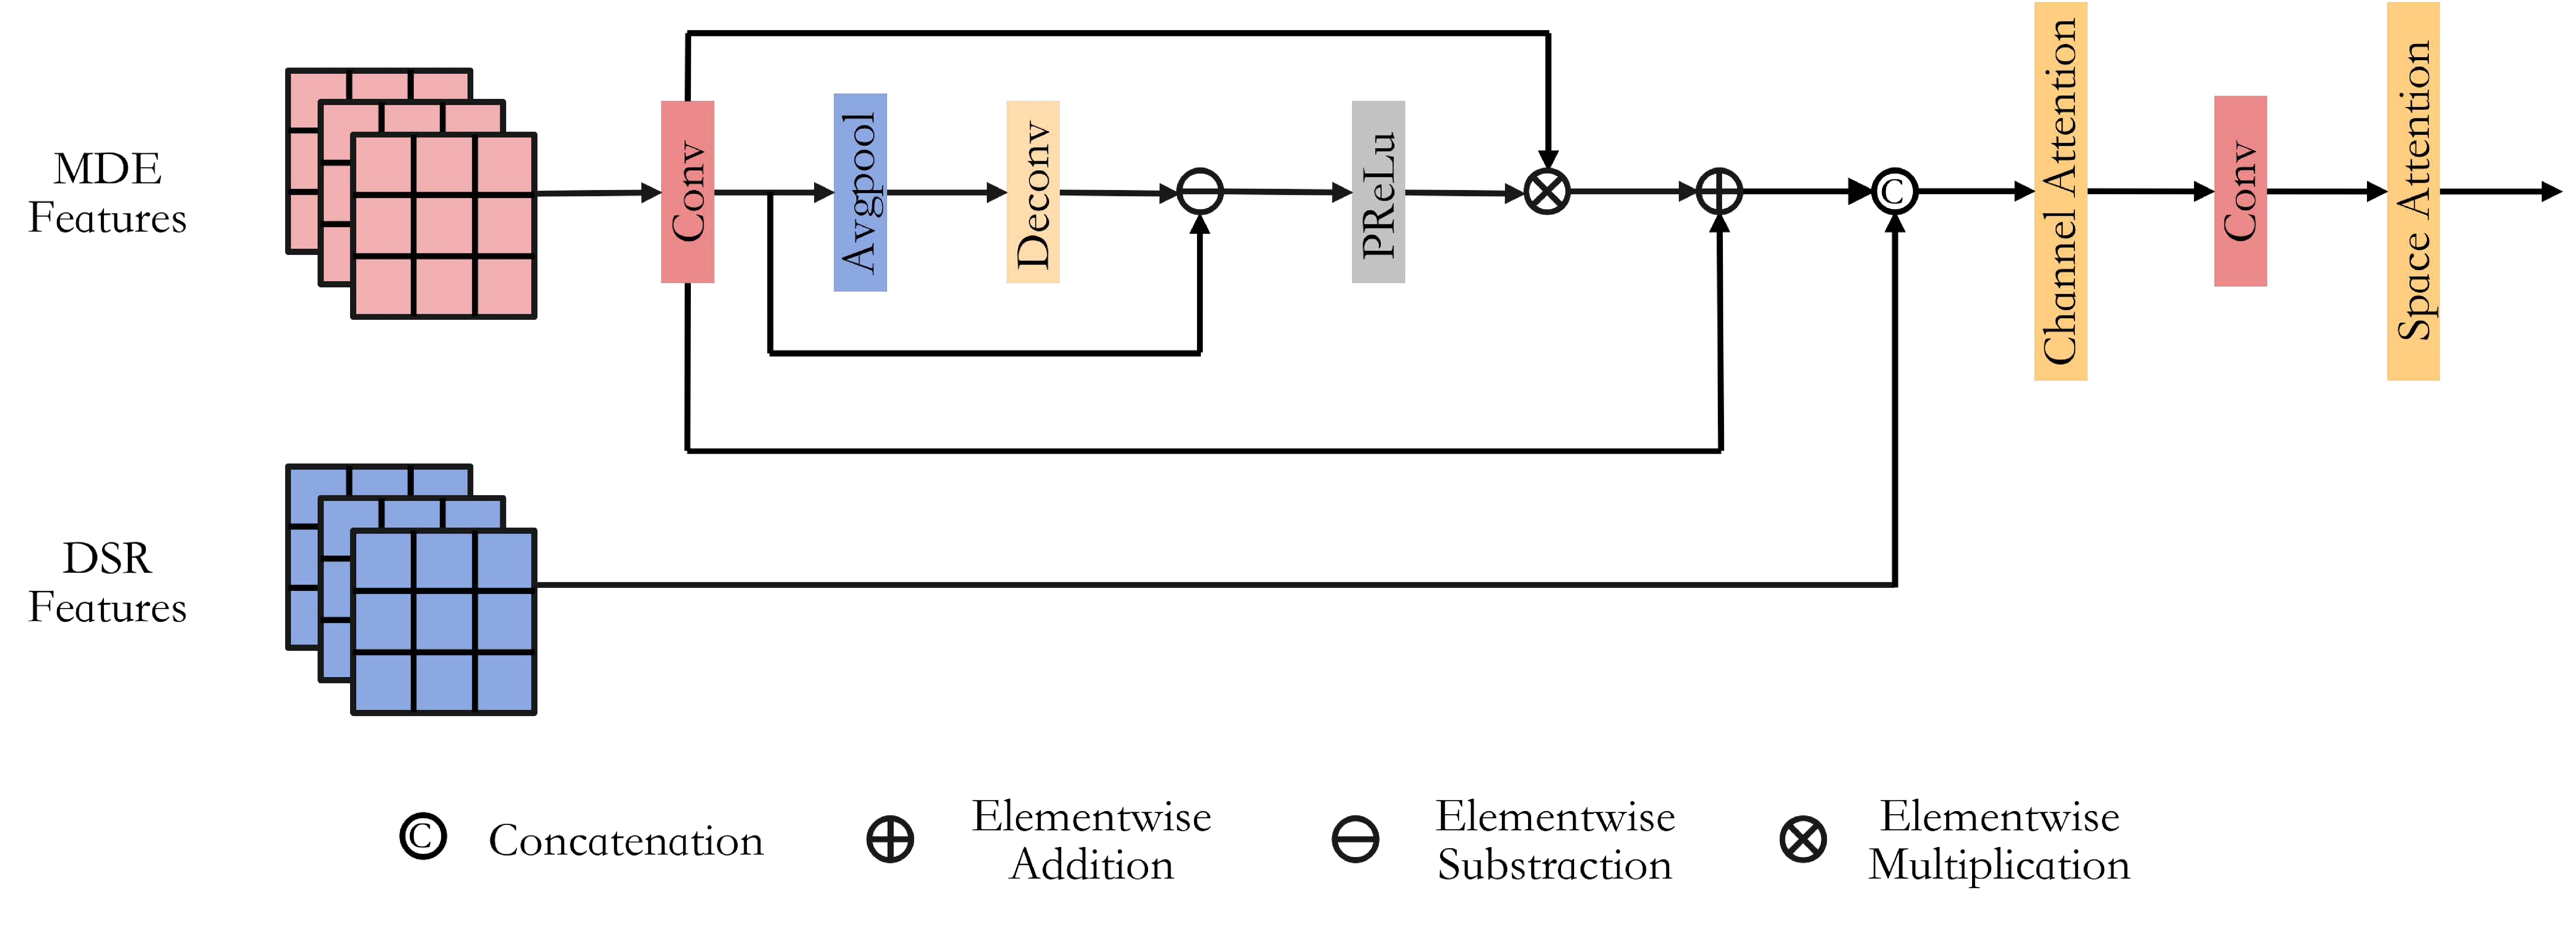
\includegraphics[width=0.55\textwidth]{figures/HABdg}}
    \subcaptionbox{Content Guidance Bridge\label{fig:g1-2}}
    {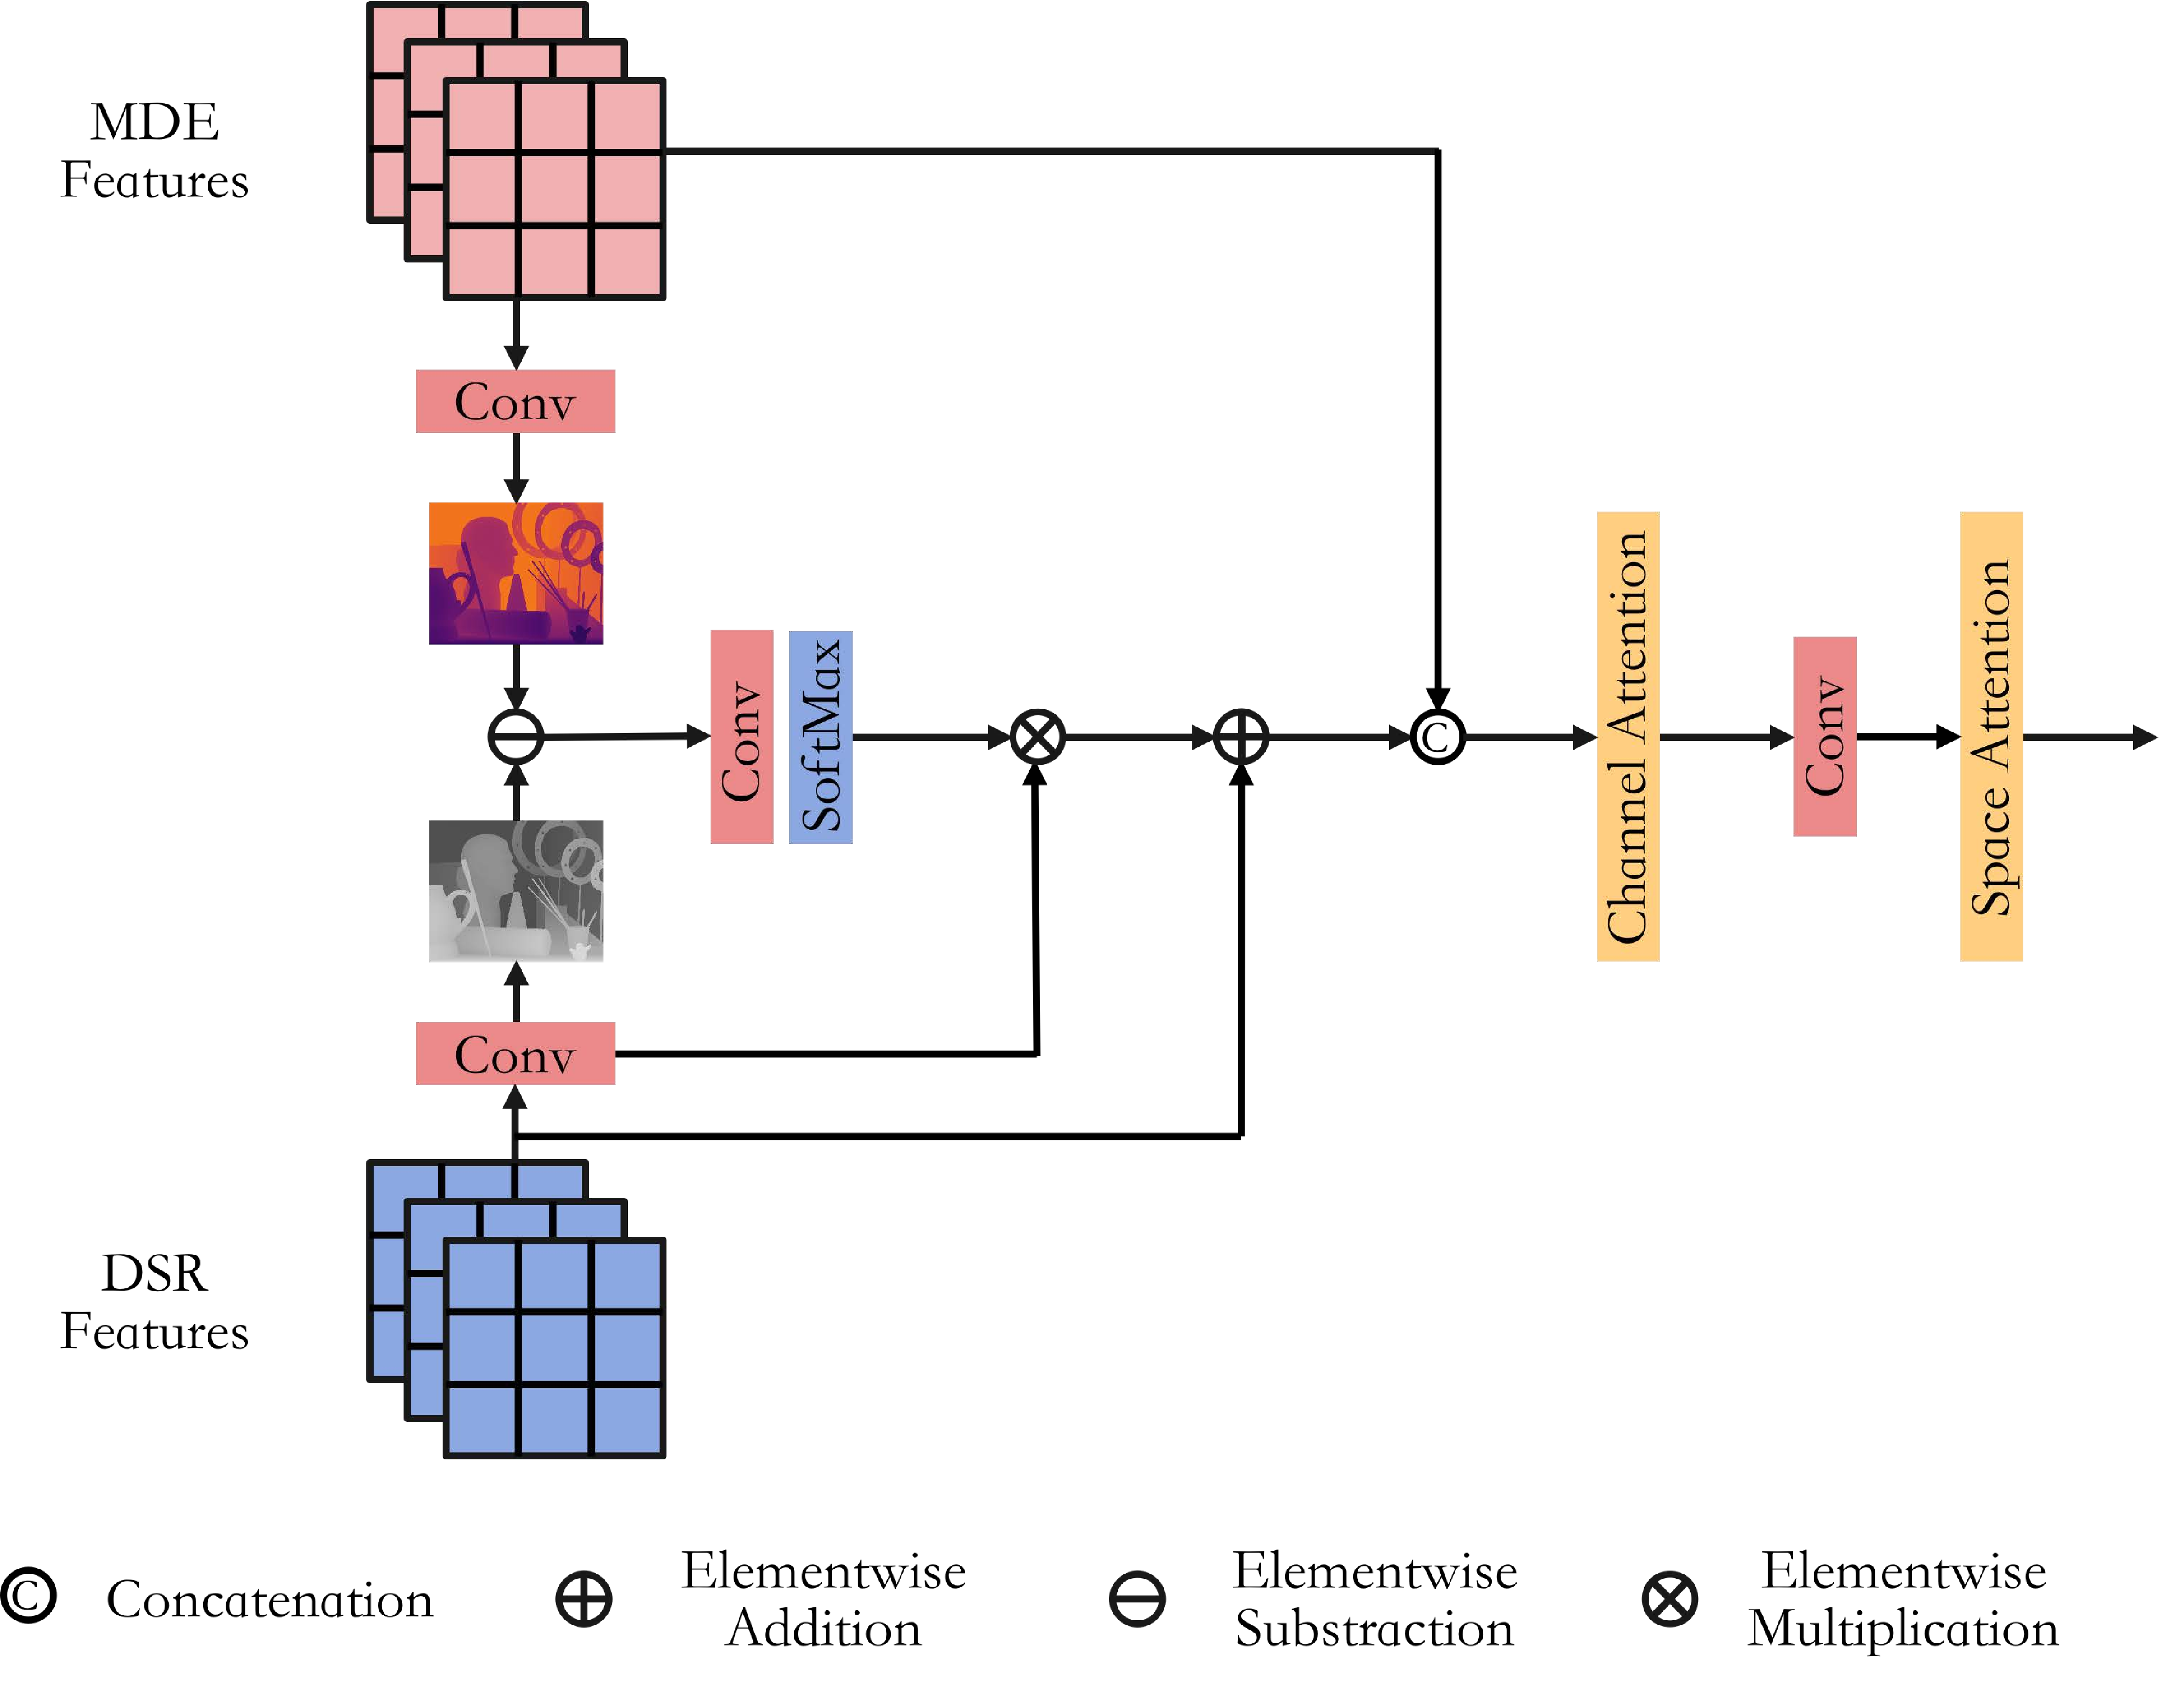
\includegraphics[width=0.4\textwidth]{figures/CGBdg}}
    \caption{桥接器示意图}\label{fig:1}
\end{figure}

\section{多行多列}
\begin{figure*}[!htbp]
  \centering
  \begin{minipage}[b]{\linewidth} 
  \subfloat[]{
    \begin{minipage}[b]{0.215\linewidth} 
      \centering
      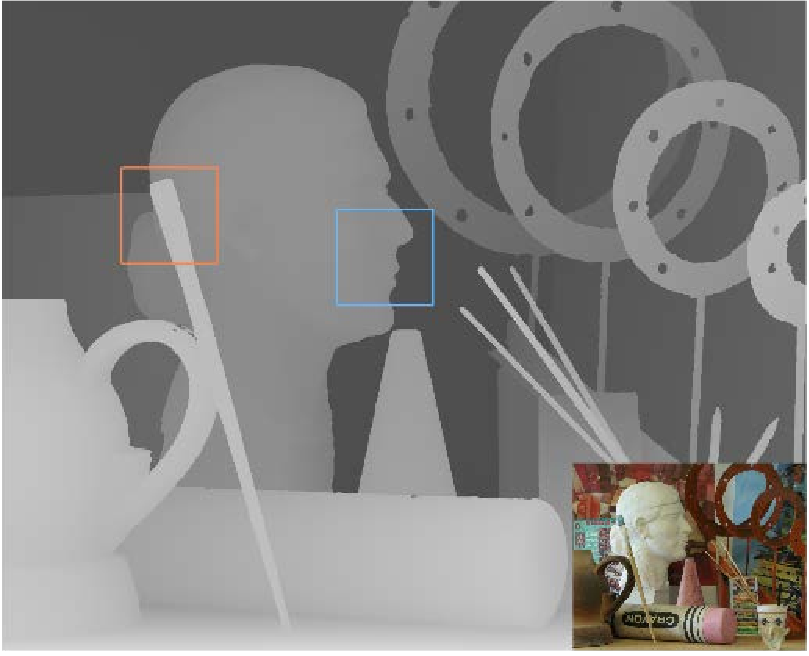
\includegraphics[width=\linewidth]{figures/art/texture.pdf}\vspace{2pt}
      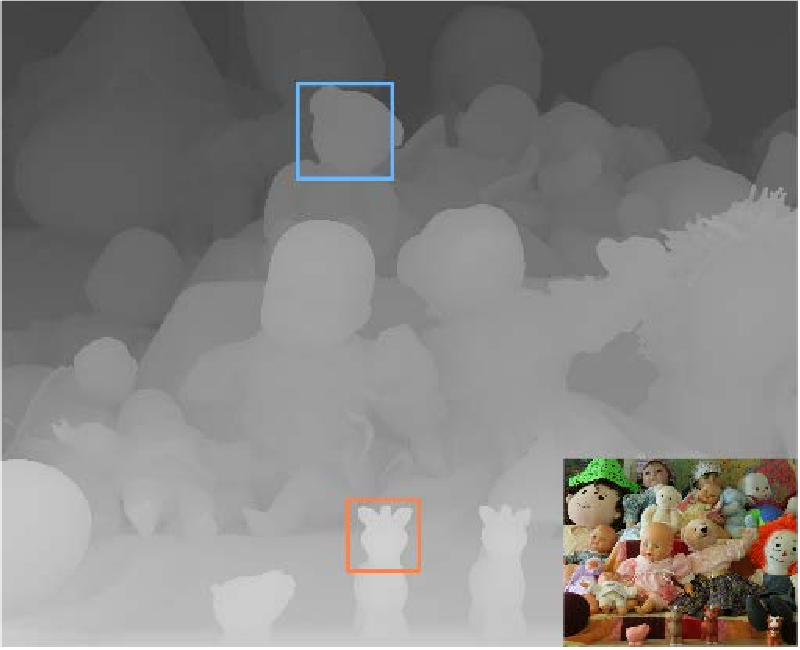
\includegraphics[width=\linewidth]{figures/doll/texture.pdf}
       \end{minipage}
  }
  \hspace{-1.2mm}	
  \subfloat[]{
    \begin{minipage}[b]{0.085\linewidth} 
      \centering
      
\includegraphics[width=\linewidth]{figures/art/lr_0.pdf}\vspace{2pt}
      
\includegraphics[width=\linewidth]{figures/art/lr_1.pdf}\vspace{2pt}
      
\includegraphics[width=\linewidth]{figures/doll/lr_0.pdf}\vspace{2pt}
      
\includegraphics[width=\linewidth]{figures/doll/lr_1.pdf}
       \end{minipage}
  }
  \hspace{-1.2mm}
    \subfloat[]{
    \begin{minipage}[b]{0.085\linewidth}
      \centering
      
\includegraphics[width=\linewidth]{figures/art/bicubic_0.pdf}\vspace{2pt}
      
\includegraphics[width=\linewidth]{figures/art/bicubic_1.pdf}\vspace{2pt}
      
\includegraphics[width=\linewidth]{figures/doll/bicubic_0.pdf}\vspace{2pt}
      
\includegraphics[width=\linewidth]{figures/doll/bicubic_1.pdf}
       \end{minipage}
  }
   \hspace{-1.2mm}
   \subfloat[]{
    \begin{minipage}[b]{0.085\linewidth}
      \centering
      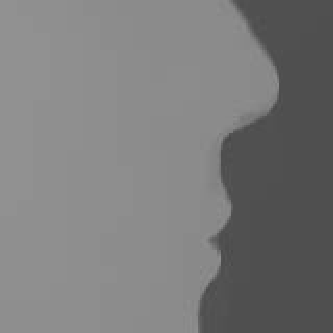
\includegraphics[width=\linewidth]{figures/art/tgv_0.pdf}\vspace{2pt}
      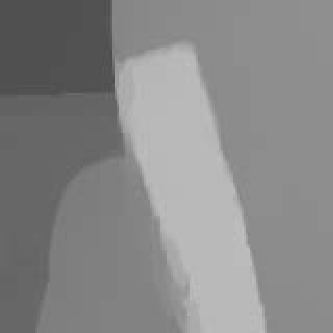
\includegraphics[width=\linewidth]{figures/art/tgv_1.pdf}\vspace{2pt}
      
\includegraphics[width=\linewidth]{figures/doll/tgv_0.pdf}\vspace{2pt}
      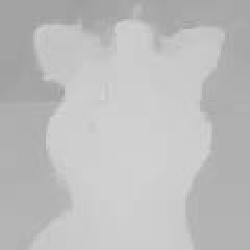
\includegraphics[width=\linewidth]{figures/doll/tgv_1.pdf}
       \end{minipage}
  }
   \hspace{-1.2mm}
  \subfloat[]{
    \begin{minipage}[b]{0.085\linewidth}
      \centering
      
\includegraphics[width=\linewidth]{figures/art/msg_0.pdf}\vspace{2pt}
      
\includegraphics[width=\linewidth]{figures/art/msg_1.pdf}\vspace{2pt}
      
\includegraphics[width=\linewidth]{figures/doll/msg_0.pdf}\vspace{2pt}
      
\includegraphics[width=\linewidth]{figures/doll/msg_1.pdf}
       \end{minipage}
  }
   \hspace{-1.2mm}
   \subfloat[]{
    \begin{minipage}[b]{0.085\linewidth}
      \centering
      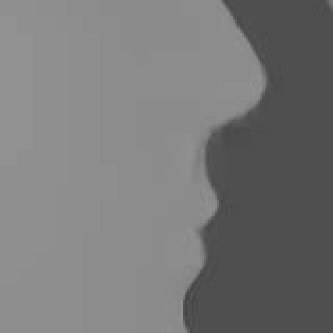
\includegraphics[width=\linewidth]{figures/art/dgdie_0.pdf}\vspace{2pt}
      
\includegraphics[width=\linewidth]{figures/art/dgdie_1.pdf}\vspace{2pt}
      
\includegraphics[width=\linewidth]{figures/doll/dgdie_0.pdf}\vspace{2pt}
      
\includegraphics[width=\linewidth]{figures/doll/dgdie_1.pdf}
       \end{minipage}
  }
   \hspace{-1.2mm}
  \subfloat[]{
    \begin{minipage}[b]{0.085\linewidth}
      \centering
      
\includegraphics[width=\linewidth]{figures/art/cvpr_0.pdf}\vspace{2pt}
      
\includegraphics[width=\linewidth]{figures/art/cvpr_1.pdf}\vspace{2pt}
      
\includegraphics[width=\linewidth]{figures/doll/cvpr_0.pdf}\vspace{2pt}
      
\includegraphics[width=\linewidth]{figures/doll/cvpr_1.pdf}
       \end{minipage}
  }
 \hspace{-1.2mm}
  \subfloat[]{
    \begin{minipage}[b]{0.085\linewidth}
      \centering
      
\includegraphics[width=\linewidth]{figures/art/ours_0.pdf}\vspace{2pt}
      
\includegraphics[width=\linewidth]{figures/art/ours_1.pdf}\vspace{2pt}
      
\includegraphics[width=\linewidth]{figures/doll/ours_0.pdf}\vspace{2pt}
      
\includegraphics[width=\linewidth]{figures/doll/ours_1.pdf}
       \end{minipage}
  }
   \hspace{-1.2mm}
    \subfloat[]{
    \begin{minipage}[b]{0.085\linewidth}
      \centering
      
\includegraphics[width=\linewidth]{figures/art/gt_0.pdf}\vspace{2pt}
      
\includegraphics[width=\linewidth]{figures/art/gt_1.pdf}\vspace{2pt}
      
\includegraphics[width=\linewidth]{figures/doll/gt_0.pdf}\vspace{2pt}
      
\includegraphics[width=\linewidth]{figures/doll/gt_1.pdf}
       \end{minipage}
  }
  \end{minipage}
  \vfill
  \caption{Visual comparisons of $\times 8$ up-sampling results on two examples (Art in the first row and Dolls in the second row). (a) Ground truth depth maps and color images; (b) LR depth patches; (c)-(h) The super-resolved depth maps generated by Bicubic, TGV, MSG, DGDIE, CTKT, and BridgeNet, respectively. (i) Ground truth. Depth patches are enlarged for clear visualization.}\label{fig:2}
\end{figure*}


\chapter{表格跨页}

\setlength{\tabcolsep}{4mm}{
\begin{longtable}{c|ccc|ccc|ccc}
\caption{Middlebury 数据集 $\times 8$ 不同超分辨率重建方法量化指标对比(一)}
\label{tab:tab4-1}\\
\toprule[1.5pt]
\multirow{2}{*}{} & \multicolumn{3}{c|}{Art} & \multicolumn{3}{c|}{Books} & \multicolumn{3}{c}{Dolls} \\\cline{2-10}
                  &  $\times 4$      &  $\times 8$      &   $\times 16$    &   $\times 4$      &     $\times 8$   &    $\times 16$    &    $\times 4$     &    $\times 8$    &    $\times 16$    \\\hline
\endfirsthead
\multicolumn{10}{c}%
{\hfill{\zihao{5} 表 \thetable\ (续)}} \\
\toprule[1.5pt]
\multirow{2}{*}{} & \multicolumn{3}{c|}{Art} & \multicolumn{3}{c|}{Books} & \multicolumn{3}{c}{Dolls} \\\cline{2-10}
                  &  $\times 4$      &  $\times 8$      &   $\times 16$    &   $\times 4$      &     $\times 8$   &    $\times 16$    &    $\times 4$     &    $\times 8$    &    $\times 16$    \\\hline
\endhead

CLMF       & 0.76 & 1.44 & 2.87       & 0.28    & 0.51   & 1.02   & 0.34    & 0.60   & 1.01   \\
JGF      & 0.47 & 0.78 & 1.54       & 0.24    & 0.43   & 0.81   & 0.33    & 0.59   & 1.06   \\
TGV         & 0.65 & 1.17 & 2.30       & 0.27    & 0.43   & 0.82   & 0.33    & 0.70   & 2.20   \\
CDLLC     & 0.53 & 0.76 & 1.41       & 0.19    & 0.46   & 0.75   & 0.31    & 0.53   & 0.79   \\
PB         & 0.79 & 0.93 & 1.98       & 0.16    & 0.43   & 0.79   & 0.53    & 0.83   & 0.99   \\
EG        & 0.48 & 0.71 & \uline{1.35}     & 0.15    & 0.36   & 0.70   & 0.27    & 0.49   & 0.74  \\\hline
SRCNN      & 0.63          & 1.21          & 2.34          & 0.25          & 0.52          & 0.97          & 0.29          & 0.58          & 1.03          \\
ATGVNet    & 0.65          & 0.81          & 1.42          & 0.43          & 0.51          & 0.79          & 0.41          & 0.52          & \textbf{0.56} \\
MSG        & 0.46          & 0.76          & 1.53          & 0.15          & 0.41          & 0.76          & 0.25          & 0.51          & 0.87          \\
DGDIE   & 0.48          & 1.20          & 2.44          & 0.30          & 0.58          & 1.02          & 0.34          & 0.63          & 0.93          \\
DEIN       & 0.40          & 0.64          & \textbf{1.34} & 0.22          & 0.37          & 0.78          & 0.22          & 0.38          & 0.73          \\
CCFN  & 0.43          & 0.72          & 1.50          & 0.17          & 0.36          & 0.69          & 0.25          & 0.46          & 0.75          \\
GSRPT     & 0.48          & 0.74          & 1.48          & 0.21          & 0.38          & 0.76          & 0.28          & 0.48          & 0.79          \\
CTKT      & \textbf{0.25} & \textbf{0.53} & 1.44          & \textbf{0.11} & \uline{0.26}    & \uline{0.67}    & \textbf{0.16} & \uline{0.36}    & 0.65          \\
BridgeNet         & \uline{0.30}    & \uline{0.58}    & 1.49          & \uline{0.14}    & \textbf{0.24} & \textbf{0.51} & \uline{0.19}    & \textbf{0.34} & \uline{0.64}   \\
\bottomrule[1.5pt]
\end{longtable}}

\setlength{\tabcolsep}{4mm}{
\begin{longtable}{c|ccc|ccc|ccc}
\caption{Middlebury 数据集 $\times 8$ 不同超分辨率重建方法量化指标对比(二)}
\label{tab:tab4-2}\\
\toprule[1.5pt]
\multirow{2}{*}{} & \multicolumn{3}{c|}{Art} & \multicolumn{3}{c|}{Books} & \multicolumn{3}{c}{Dolls} \\\cline{2-10}
                  &  $\times 4$      &  $\times 8$      &   $\times 16$    &   $\times 4$      &     $\times 8$   &    $\times 16$    &    $\times 4$     &    $\times 8$    &    $\times 16$    \\\hline
\endfirsthead
\multicolumn{10}{c}%
{\hfill{\zihao{5} 表 \thetable\ (续)}} \\
\toprule[1.5pt]
\multirow{2}{*}{} & \multicolumn{3}{c|}{Art} & \multicolumn{3}{c|}{Books} & \multicolumn{3}{c}{Dolls} \\\cline{2-10}
                  &  $\times 4$      &  $\times 8$      &   $\times 16$    &   $\times 4$      &     $\times 8$   &    $\times 16$    &    $\times 4$     &    $\times 8$    &    $\times 16$    \\\hline
\endhead

CLMF      & 0.50 & 0.80       & 1.67          & 0.29 & 0.51 & 0.97 & 0.51 & 0.84 & 1.55          \\ 
JGF     & 0.36 & 0.64       & 1.20          & 0.25 & 0.46 & 0.80 & 0.38 & 0.64 & 1.09          \\ 
TGV       & 0.55 & 1.22       & 3.37          & 0.29 & 0.49 & 0.90 & 0.49 & 1.03 & 3.05          \\ 
CDLLC    & 0.30 & 0.48       & 0.96          & 0.27 & 0.46 & 0.79 & 0.43 & 0.55 & 0.98          \\ 
PB       & 1.13 & 1.89       & 2.87          & 0.17 & 0.47 & 0.82 & 0.56 & 0.97 & 1.89          \\ \bottomrule[1.5pt]
EG       & 0.28 & 0.45       & \uline{0.92}    & 0.23 & 0.42 & 0.75 & 0.36 & 0.51 & 0.95          \\ 
\hline
SRCNN   & 0.40 & 0.87       & 1.74          & 0.25 & 0.43 & 0.87 & 0.35 & 0.75 & 1.47          \\
ATGVNet  & 0.37 & 0.89       & 0.94          & 0.38 & 0.45 & 0.80 & 0.41 & 0.58 & 1.01 \\
MSG    & 0.30 & 0.46       & 1.12          & 0.21 & 0.43 & 0.76 & 0.31 & 0.52 & 0.99          \\
DGDIE    & 0.35 & 0.86       & 1.56          & 0.28 & 0.58 & 0.98 & 0.35 & 0.73 & 1.29          \\
DEIN       & 0.23 & \uline{0.36} & 0.81 & 0.20 & 0.35 & 0.73 & 0.26 & 0.40 & 0.80          \\
CCFN   & 0.24 & 0.41       & 0.71          & 0.23 & 0.39 & 0.73 & 0.29 & 0.46 & 0.95          \\
GSRPT   & 0.33 & 0.56       & 1.24          & 0.24 & 0.49 & 0.80 & 0.31 & 0.61 & 1.07          \\
CTKT     & \textbf{0.16} & \uline{0.36}    & \uline{0.76}    & \textbf{0.13} & \uline{0.27}    & \uline{0.69}    & \textbf{0.17} & \uline{0.35}    & \uline{0.77}          \\
BridgeNet         & \uline{0.17}    & \textbf{0.34} & \textbf{0.71} & \uline{0.15}    & \textbf{0.26} & \textbf{0.54} & \uline{0.19}    & \textbf{0.31} &  \textbf{0.70}\\
\bottomrule[1.5pt]
\end{longtable}}


\chapter{算法代码}

\begin{adjustbox}{height=\the\paperheight-19cm,width=0.8\linewidth} 
\begin{algorithm}[H]
        \caption{Joint Learning Strategy}
        \LinesNumbered
        \KwIn{Training data $D_{LR}$, $I_{HR}$, $D_{HR}$}
        \KwOut{$D_{SR}$, $D_{DE}$}
        Randomly initialize DSRNet and MDENet\\
       
        \For{ epoch=1; epoch $\leq$ 400;}
        {
         ——————————————— Step 1 ———————————————\\
        $F_{MDE}=Encoder_{MDE}(I_{HR}^n)$\\
        $F_{DSR}^{shallow}=Res^{(2)}(conv(D_{LR}))$ \tcp*{shallow feature extraction}
        \For(\tcp*[f]{ i refers to $i^{th}$ layer of encoder}){i=1; i $\leq$ 3} 
        {
        \If{i=1}
        {
        $Fe_{DSR}^i=maxpool(Res^{(4)}(F_{DSR}^{shallow}))$\\
        }
        \Else{
        $Fe_{DSR}^i=maxpool(Res^{(4)}(F_{ha}^{i-1}))$\\
        }
        $F_{blurred}^i=deconv(avgpool(F_{MDE}^i)$\\
        $A_{hf}^i=PRelu(F_{MDE}^i-F_{blurred}^i)$\\
        $F_{hg}^i=F_{MDE}^i+A_{hf}^i\cdot F_{MDE}^i$\\
        $F_{comp}^i=[Fe_{DSR}^i,F_{hg}^i]$\\
        $F_{ha}^i=SA(conv_{1\times 1}(CA(F_{comp}^i)))$\\
        }
        $F_{DSR}^{deeper}=Res^{(32)}(F_{ha}^3)$\\
        $F_{DSR}^{multi-scale}=conv(conv(conv(Fe_{DSR}^{shallow}+Fe_{DSR}^1)+F_{DSR}^2)+Fe_{DSR}^3)$\tcp*{multi-scale features fusion}
        $F_{DSR}^{fusion}=Res^{(2)}(F_{DSR}^{deeper}+F_{DSR}^{multi-scale})$\\
        $F_{DSR}^{low-freq}=Downsample(F_{DSR}^{shallow})$\\
        \For(\tcp*[f]{ j refers to $j^{th}$ layer of decoder}){i=1; i $\leq$ 3} 
        {
        \If{i=1}
        {
        $Fd_{DSR}^j=pixelshuffle(conv(F_{DSR}^{fusion}+F_{DSR}^{low-freq}))$\\
        }
        \Else{
        $Fd_{DSR}^j=pixelshuffle(conv(F_{DSR}^{j-1}))$\\
        }
        }
        $D_{SR}=conv_{1 \times 1}(Fd_{DSR}^3)$\\
        Update weights of parts related to DSR with $\mathcal{L}_{DSR}=||D_{SR}-D_{HR}||_1$\\
        ——————————————— Step 2 ———————————————\\
        $F_{MDE}=Encoder_{MDE}(I_{HR}^n)$\\
        \For{k=1;k $\leq$ 4}
        {
        \If{k=1}
        {
        $Fp_{MDE}^k=conv(Fe_{MDE}^{5-k})$
        }
        \Else
        {
        $Fe_{MDE}^{5-k}=interpolate(Fe_{MDE}^{5-k})$\\
        $Fp_{MDE}^k= conv(Fe_{MDE}^{5-k} +Fe_{MDE}^{5-(k+1)})$
        }
        }
         
        \For{j=1;k $\leq$ 3}
        {
        \If{j=1}
        {
        $Fd_{MDE}^j=CLIFF(Fp_{MDE}^1,Fp_{MDE}^2)$\\
        }
        \Else
        {
        $M_{DSR}^j=conv_{1\times1}(Fd_{DSR}^j)$\\
        $M_{MDE}^j=conv_{1\times1}(Fd_{MDE}^j)$\\
        $W_{diff}^j=softmax(conv_{1\times1}(M_{DSR}^j-M_{MDE}^j))$\\
        $F_{ca}^j=Fd_{DSR}^j+W_{diff}^j\ast Fd_{DSR}^j$\\
        $F_{con}^j=[Fd_{MDE}^j,F_{ca}^j]$\\
        $F_{cg}^j=SA(conv_{1\times1}(CA(F_{con}^j)))$\\
        $Fd_{MDE}^j=CLIFF(F_{cg}^j,Fp_{MDE}^{j+1})$\\
        }
        }
        $D_{DE}=interpolate(conv_{1\times 1}(Fd_{MDE}^3))$\\
        Update weights of parts related to MDE with $\mathcal{L}_{MDE}=||D_{DE}-D_{HR}||_1$
        }
    \end{algorithm}
\end{adjustbox}

%\lstinputlisting[language=Python,firstline=1,lastline=178]{code/edsrx2.py}

%========================================================================%
% 参考文献
%========================================================================%
\newpage
\pagestyle{bjtufancy}

\nocite{*} % 显示.bib文件中的所有参考文献,无论正文是否引用

\printbibliography[heading=bjtuheading]
\addcontentsline{toc}{part}{参考文献}
\cleardoublepage
%========================================================================%
% 致谢
%========================================================================%
%\thankspage
\begin{thanks}
[鼠标左键单击选择该段落,输入替换之。内容为小四号宋或楷体字。] 放置在参考文献页后,对象包括:1)国家科学基金,资助研究工作的奖学金基金,合同单位,资助或支持的企业、组织或个人。2)协助完成研究工作和提供便利条件的组织或个人。3)在研究工作中提出建议和提供帮助的人。4)给予转载和引用权的资料、图片、文献、研究思想和设想的所有者。5)其他应感谢的组织和个人。
\end{thanks}
%========================================================================%
% 附录
%========================================================================%
\begin{appendix}

\section*{附录A\hspace{1em}程序代码【1级标题,三号黑体字】}
\zihao{5} 
附录是作为论文主体的补充项目,并不是必须的。\par
论文的附录依序用大写正体英文字母A、B、C……编序号,如:附录A。

\section*{附录B\hspace{1em}工程图纸【1级标题,三号黑体字】}

\end{appendix}

\end{document}
